\subsection{Improve workflow with branching}
Up to this point, only some basic activities of the version control software have been
demonstrated like saving changes to the project files and displaying history of changes. No branching
has been done, however, it is more important feature when it comes to complex development project, faster iteration cycles and
CI/CD principles. In this section, a new development branch (stream in Perforce's terminology) is created beside the one
called main and all incremental development is done to the development branch which is later merged to the main one.
\subsubsection{Setup new stream}
steps to setup streams in Perforce
\begin{figure}[H]
    \centering
    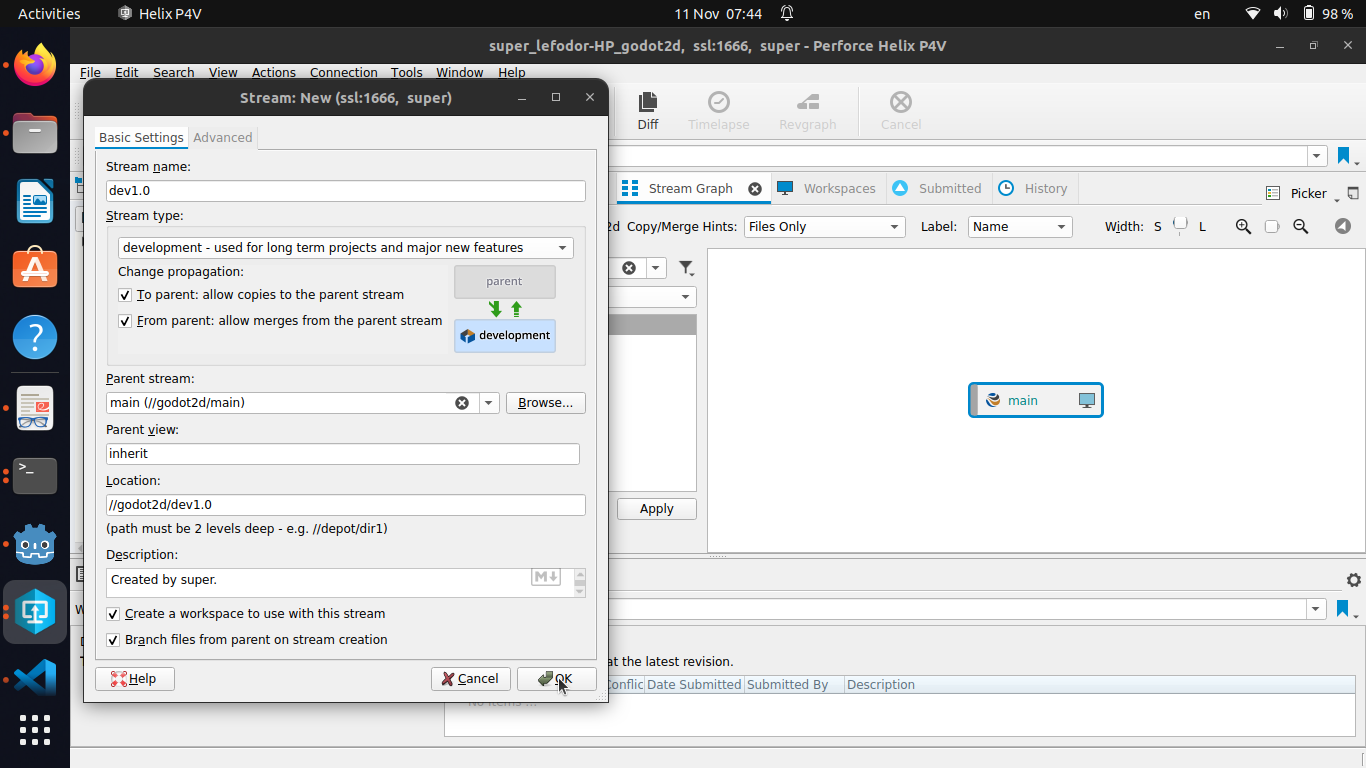
\includegraphics[width=\textwidth]{new-stream-for-branching.png}
    \caption{p4v new stream for branching}
    \label{fig:new-stream-for-branching}
\end{figure}
A new development stream (branch) has been created:
\begin{figure}[H]
    \centering
    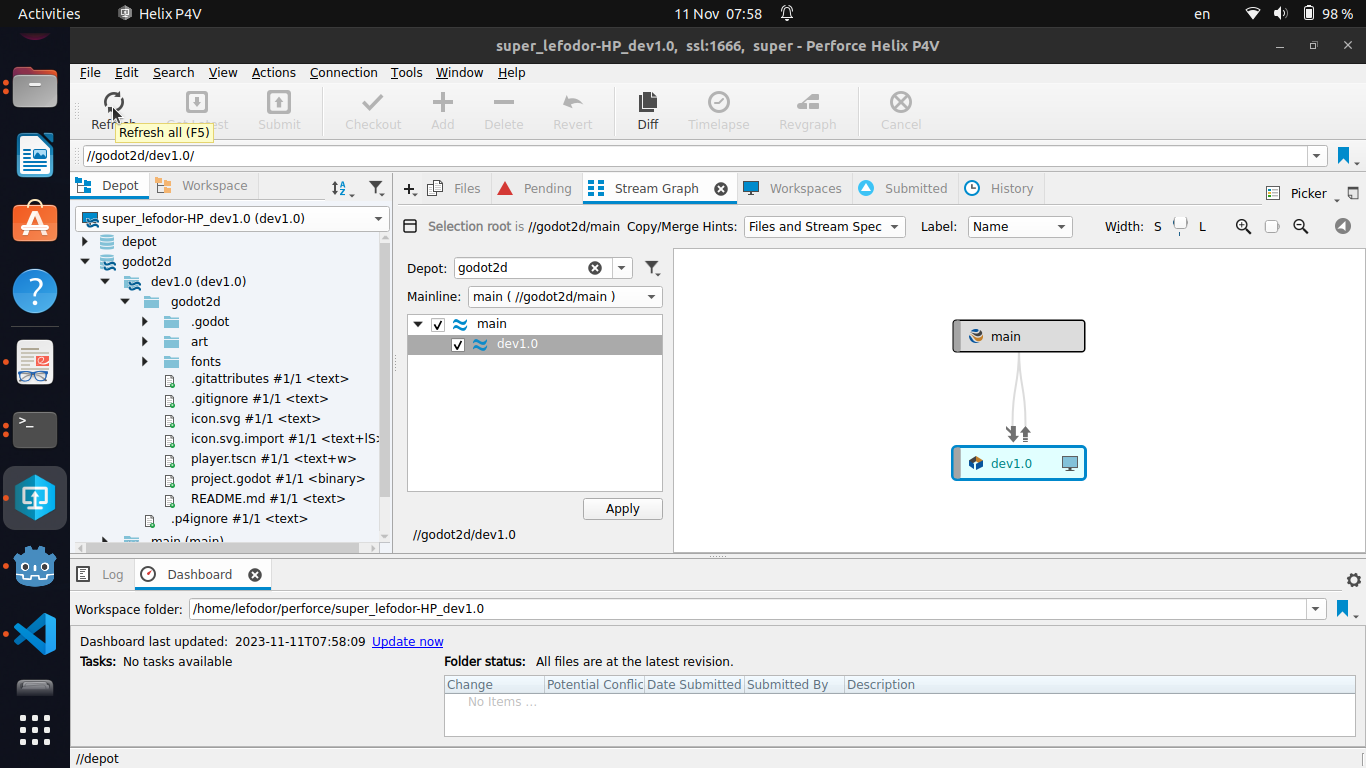
\includegraphics[width=\textwidth]{new-branch-dev1.0.png}
    \caption{new stream (branch) dev1.0}
    \label{fig:new-branch-dev1.0}
\end{figure}
From this point onwards, all changes are to be made on the development stream and later merged back to the more stable
main stream. Also, changes need to be made to the workspace related to this branch and not on the one linked to main.

\subsection{Coding the player scene and creating the enemy}
%\begin{enumerate}[resume]
  %\item 
  \href{https://docs.godotengine.org/en/stable/getting_started/first_2d_game/03.coding_the_player.html}{\color{blue}Coding player scene}. 
  Add script to player by selecting the scene and click on the "Attach Script" button.
  \begin{figure}[H]
    \centering
    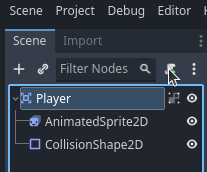
\includegraphics[scale=0.5]{add-script-to-player.png}
    \caption{add script to player}
    \label{fig:add-script-to-player}
  \end{figure}
  The added script (\textit{player.gd}) should look like as below:
  \begin{verbatim}
    extends Area2D

    signal hit

    @export var speed = 400 # How fast the player will move (pixels/sec).
    var screen_size # Size of the game window.
    
    # Called when the node enters the scene tree for the first time.
    func _ready():
      screen_size = get_viewport_rect().size
    
    
    # Called every frame. 'delta' is the elapsed time since the previous frame.
    func _process(delta):
      var velocity = Vector2.ZERO # The player's movement vector.
      if Input.is_action_pressed("ui_right"):
        velocity.x += 1
      if Input.is_action_pressed("ui_left"):
        velocity.x -= 1
      if Input.is_action_pressed("ui_down"):
        velocity.y += 1
      if Input.is_action_pressed("ui_up"):
        velocity.y -= 1
    
      if velocity.length() > 0:
        velocity = velocity.normalized() * speed
        $AnimatedSprite2D.play()
      else:
        $AnimatedSprite2D.stop()
      
      if velocity.x != 0:
        $AnimatedSprite2D.animation = "walk"
        $AnimatedSprite2D.flip_v = false
        # See the note below about boolean assignment.
        $AnimatedSprite2D.flip_h = velocity.x < 0
      elif velocity.y != 0:
        $AnimatedSprite2D.animation = "up"
        $AnimatedSprite2D.flip_v = velocity.y > 0
      
      position += velocity * delta
      position = position.clamp(Vector2.ZERO, screen_size)  
      
    func _on_body_entered(_body):
      hide() # Player disappears after being hit.
      hit.emit()
      # Must be deferred as we can't change physics properties on a physics callback.
      $CollisionShape2D.set_deferred("disabled", true)
      
    func start(pos):
      position = pos
      show()
      $CollisionShape2D.disabled = false
  \end{verbatim} 
  After this step, it is already possible to run the game by pressing F6 and use the arrow buttons to control the player's
  character up/down and left/right.
  Final step of this point is the preparation for collisions. The \textit{signal hit} line generates a so called signal.
  Signals are emitted upon certain events, in this case, when the player gets hit.
  \begin{figure}[H]
    \centering
    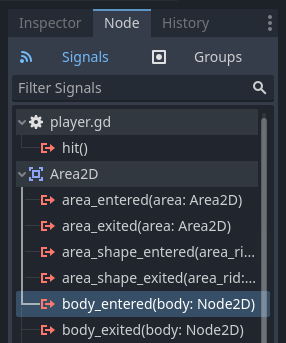
\includegraphics[scale=0.5]{player-signals.png}
    %\setlength{\belowcaptionskip}{-15pt}
    \caption{player signals}
    \label{fig:player-signals}
  \end{figure}
  The \textit{body\_entered} signal is connected to the player meaning that if an Area2D object hits the player the signal
  is emitted. By connecting the signal, a function is created (\textit{func \_on\_body\_entered}) in the script file that defines the behaviour upon signal
  emission. The final piece of code (\textit{func start()}) defines the starting position of the player when the game starts.
%\end{enumerate}
The next step in the version control is to merge changes in stream \textit{dev1.0} back to the \textit{main} stream. Currently,
the Stream Graph in P4V looks like this.
\begin{figure}[H]
  \centering
  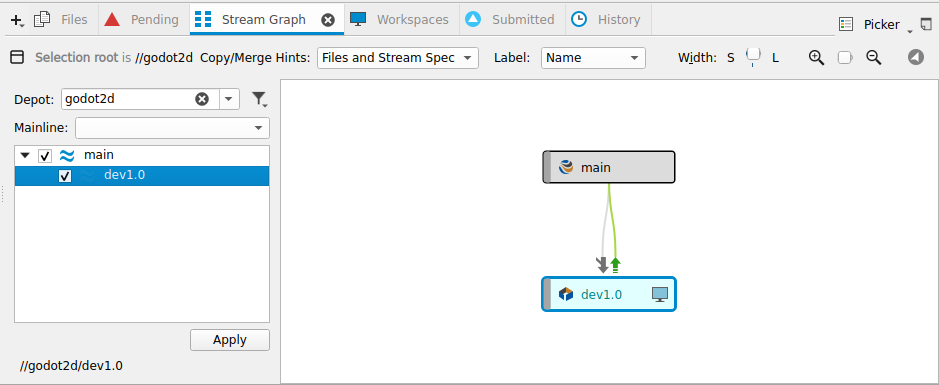
\includegraphics[width=\textwidth]{copy-dev-to-main.png}
  \caption{copy files from dev to main}
  \label{fig:copy-dev-to-main}
\end{figure}
The green arrow means merge or copy operation is available. As for the terminology, "merge" means send changes from the 
more stable stream (main) to the less stable one (dev) and "copy" means vica versa. This case, only the less stable stream
\textit{dev} stream is changed, so only copy operation is needed. Gray arrow means no copy or merge operations are necessary.
Right click on the target stream {$=>$} \textit{Copy files to main}. In the popup window, the workspace for the target stream
has to be activated then click on \textit{Copy} to copy the files. Finally, the in the main stream, the changes from the 
copy operation has to be submitted. With these steps, changes from the development branch are also saved in the main branch
and branches are synchronised.
%\begin{enumerate}[resume]
  %\item 
  \href{https://docs.godotengine.org/en/stable/getting_started/first_2d_game/04.creating_the_enemy.html}{\color{blue}Creating the enemy}
  Create enemy scene. Add behaviour and movement.
  Create a new scene called "Mob", which will be instanced as many times as wished, in random locations of the screen and 
  move in randomly selected directions. Click \textbf{Scene} {$=>$} \textbf{New Scene} and add the following structure:
  \begin{itemize}
    \item RigidBody2D (called Mob)
      \begin{itemize}
        \item AnimatedSprite2D
        \item CollisionShape2D
        \item VisibleOnScreenNotifier2D
      \end{itemize}
  \end{itemize}
  \begin{figure}[H]
    \centering
    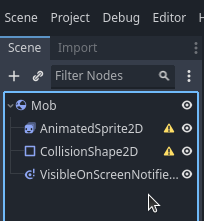
\includegraphics[scale=0.5]{create-enemy.png}
    \caption{create enemy}
    \label{fig:create-enemy}
  \end{figure}
Select the Mob scene and set the to \textit{Gravity scale} in the \textit{Inspector} tab to 0. 
In section \textit{CollisionObject2D}, under \textbf{Collision}, in property \textbf{Mask} uncheck the 1.
Setup the animation for the enemy similarly as in \ref{animation}. There are three animations to be defined:
\textit{fly}, \textit{swim} and \textit{walk}. Drag the corresponding sprites for each of them, set the FPS to 3.
In the \textit{Inspector} window, under \textbf{Node2D/Transform}, set \textit{Rotation} to 90 and \textit{Scale}
to 0.75.
\begin{figure}[H]
  \centering
  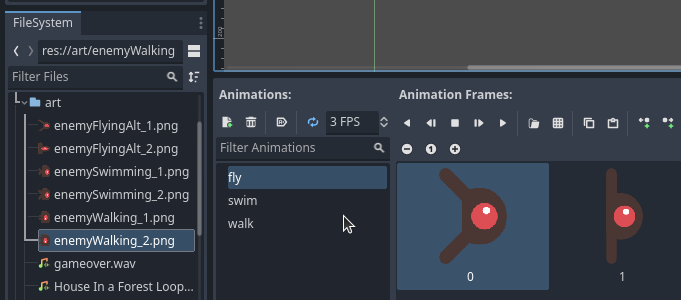
\includegraphics[scale=0.5]{animation-enemy.png}
  %\setlength{\belowcaptionskip}{-12pt}
  \caption{animation enemy}
  \label{fig:animation-enemy}
\end{figure}
Finally, define \textit{CapsuleShape} for the collision shape's \textit{Shape} property. Add a ew script to the Mob scene
with the below content and save the script as \textit{mob.gd}:
\begin{verbatim}
  extends RigidBody2D


  # Called when the node enters the scene tree for the first time.
  func _ready():
	  var mob_types = $AnimatedSprite2D.sprite_frames.get_animation_names()
	  $AnimatedSprite2D.play(mob_types[randi() % mob_types.size()])


  # Called every frame. 'delta' is the elapsed time since the previous frame.
  func _process(_delta):
	  pass

  func _on_visible_on_screen_enabler_2d_screen_exited():
	  queue_free()
\end{verbatim}
%\end{enumerate}
Regarding P4V, same steps have to be done as previously when player scene and script were added (add new files,
submit changes and copy files from dev stream if sync is needed at this moment). The \textit{dev} workspace looks as 
follows after creating and adding the enemy.
\begin{figure}[H]
  \centering
  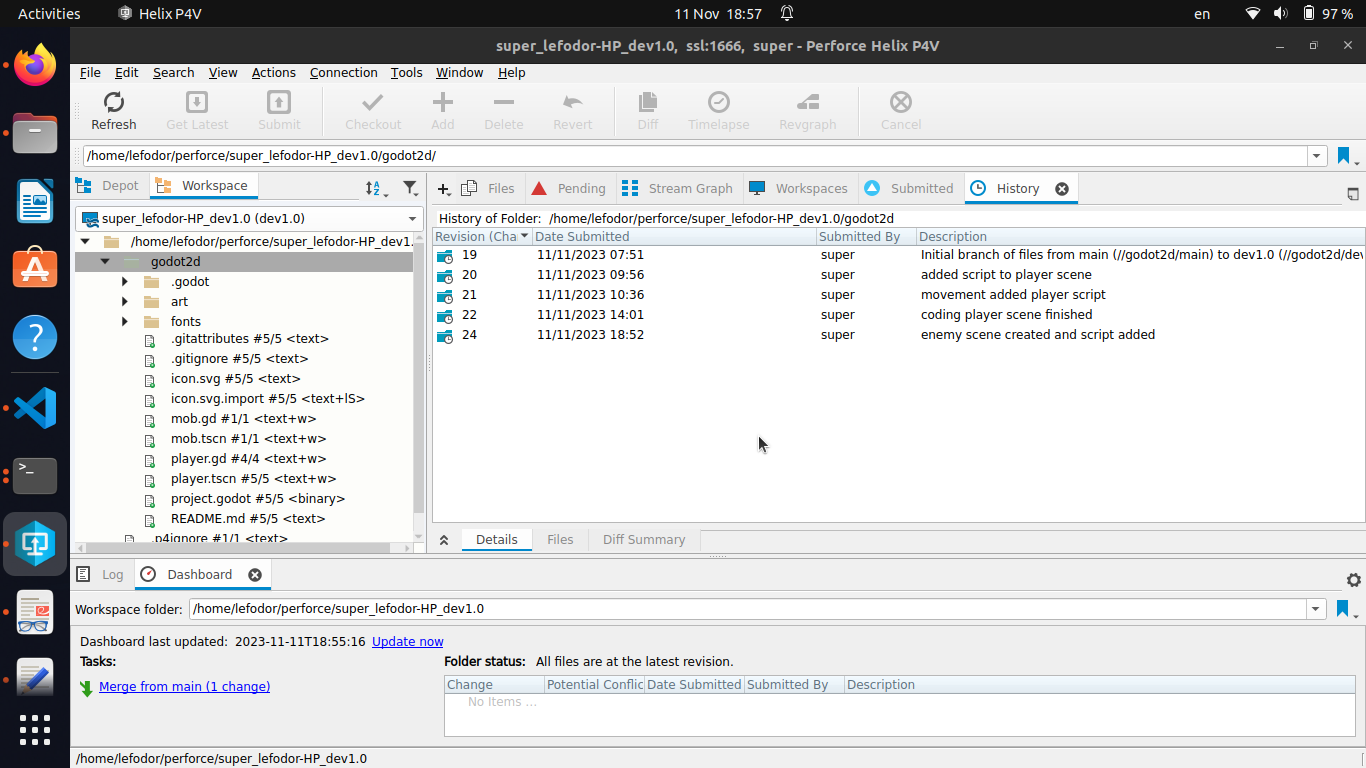
\includegraphics[width=\textwidth]{workspace-after-enemy-creation.png}
  \caption{workspace after enemy creation}
  \label{fig:workspace-after-enemy-creation}
\end{figure}